\documentclass[parskip]{scrartcl}


\RequirePackage[english]{babel}
\RequirePackage{graphicx}
\RequirePackage{hyperref}

\title{Assignment 4: Renting Costs in Stuttgart}
\author{Grzegorz Lippe}
\date{\today}

\begin{document}

\maketitle

\begin{abstract}
    This is the final Assignment in the Coursera course ``Applied Plotting,
    Charting \& Data Representation in Python''. I do not mind if Coursera
    shares this solution.
\end{abstract}

\section{Region and Domain}

Stuttgart, Baden-W\"urttemberg, Germany\\
Cost of Living / Inflation

\section{Research Question}

Is the increasing population, or the decreasing availability of living space in
Stuttgart responsible for the increasing of the renting costs?

\section{Links}

\begin{itemize}
    \item The data for the amount of houses and flats in Stuttgart:
    \href{https://www.statistik-bw.de/Wohnen/WkostenVerhaeltnis/99045041.tab?R=KR111}{Statistik-BW},
    an website with table elements, that were downloaded with \texttt{pandas.read\_html()}.
    \item The data for the population of Stuttgart:
    \href{https://www.statistik-bw.de/BevoelkGebiet/Bevoelkerung/01515020.tab?R=KR111}{Statistik-BW},
    the same source like in the first link.
    \item The data for the rent prices in Stuttgart:
    \href{https://de.statista.com/statistik/daten/studie/535218/umfrage/mietpreise-auf-dem-wohnungsmarkt-in-stuttgart}{Statista},
    this website provides the possibility to manually download an Excel file,
    which then was imported with \texttt{pandas.read\_excel()}.
\end{itemize}

\newpage

\section{Image}

\begin{figure}[ht!]
    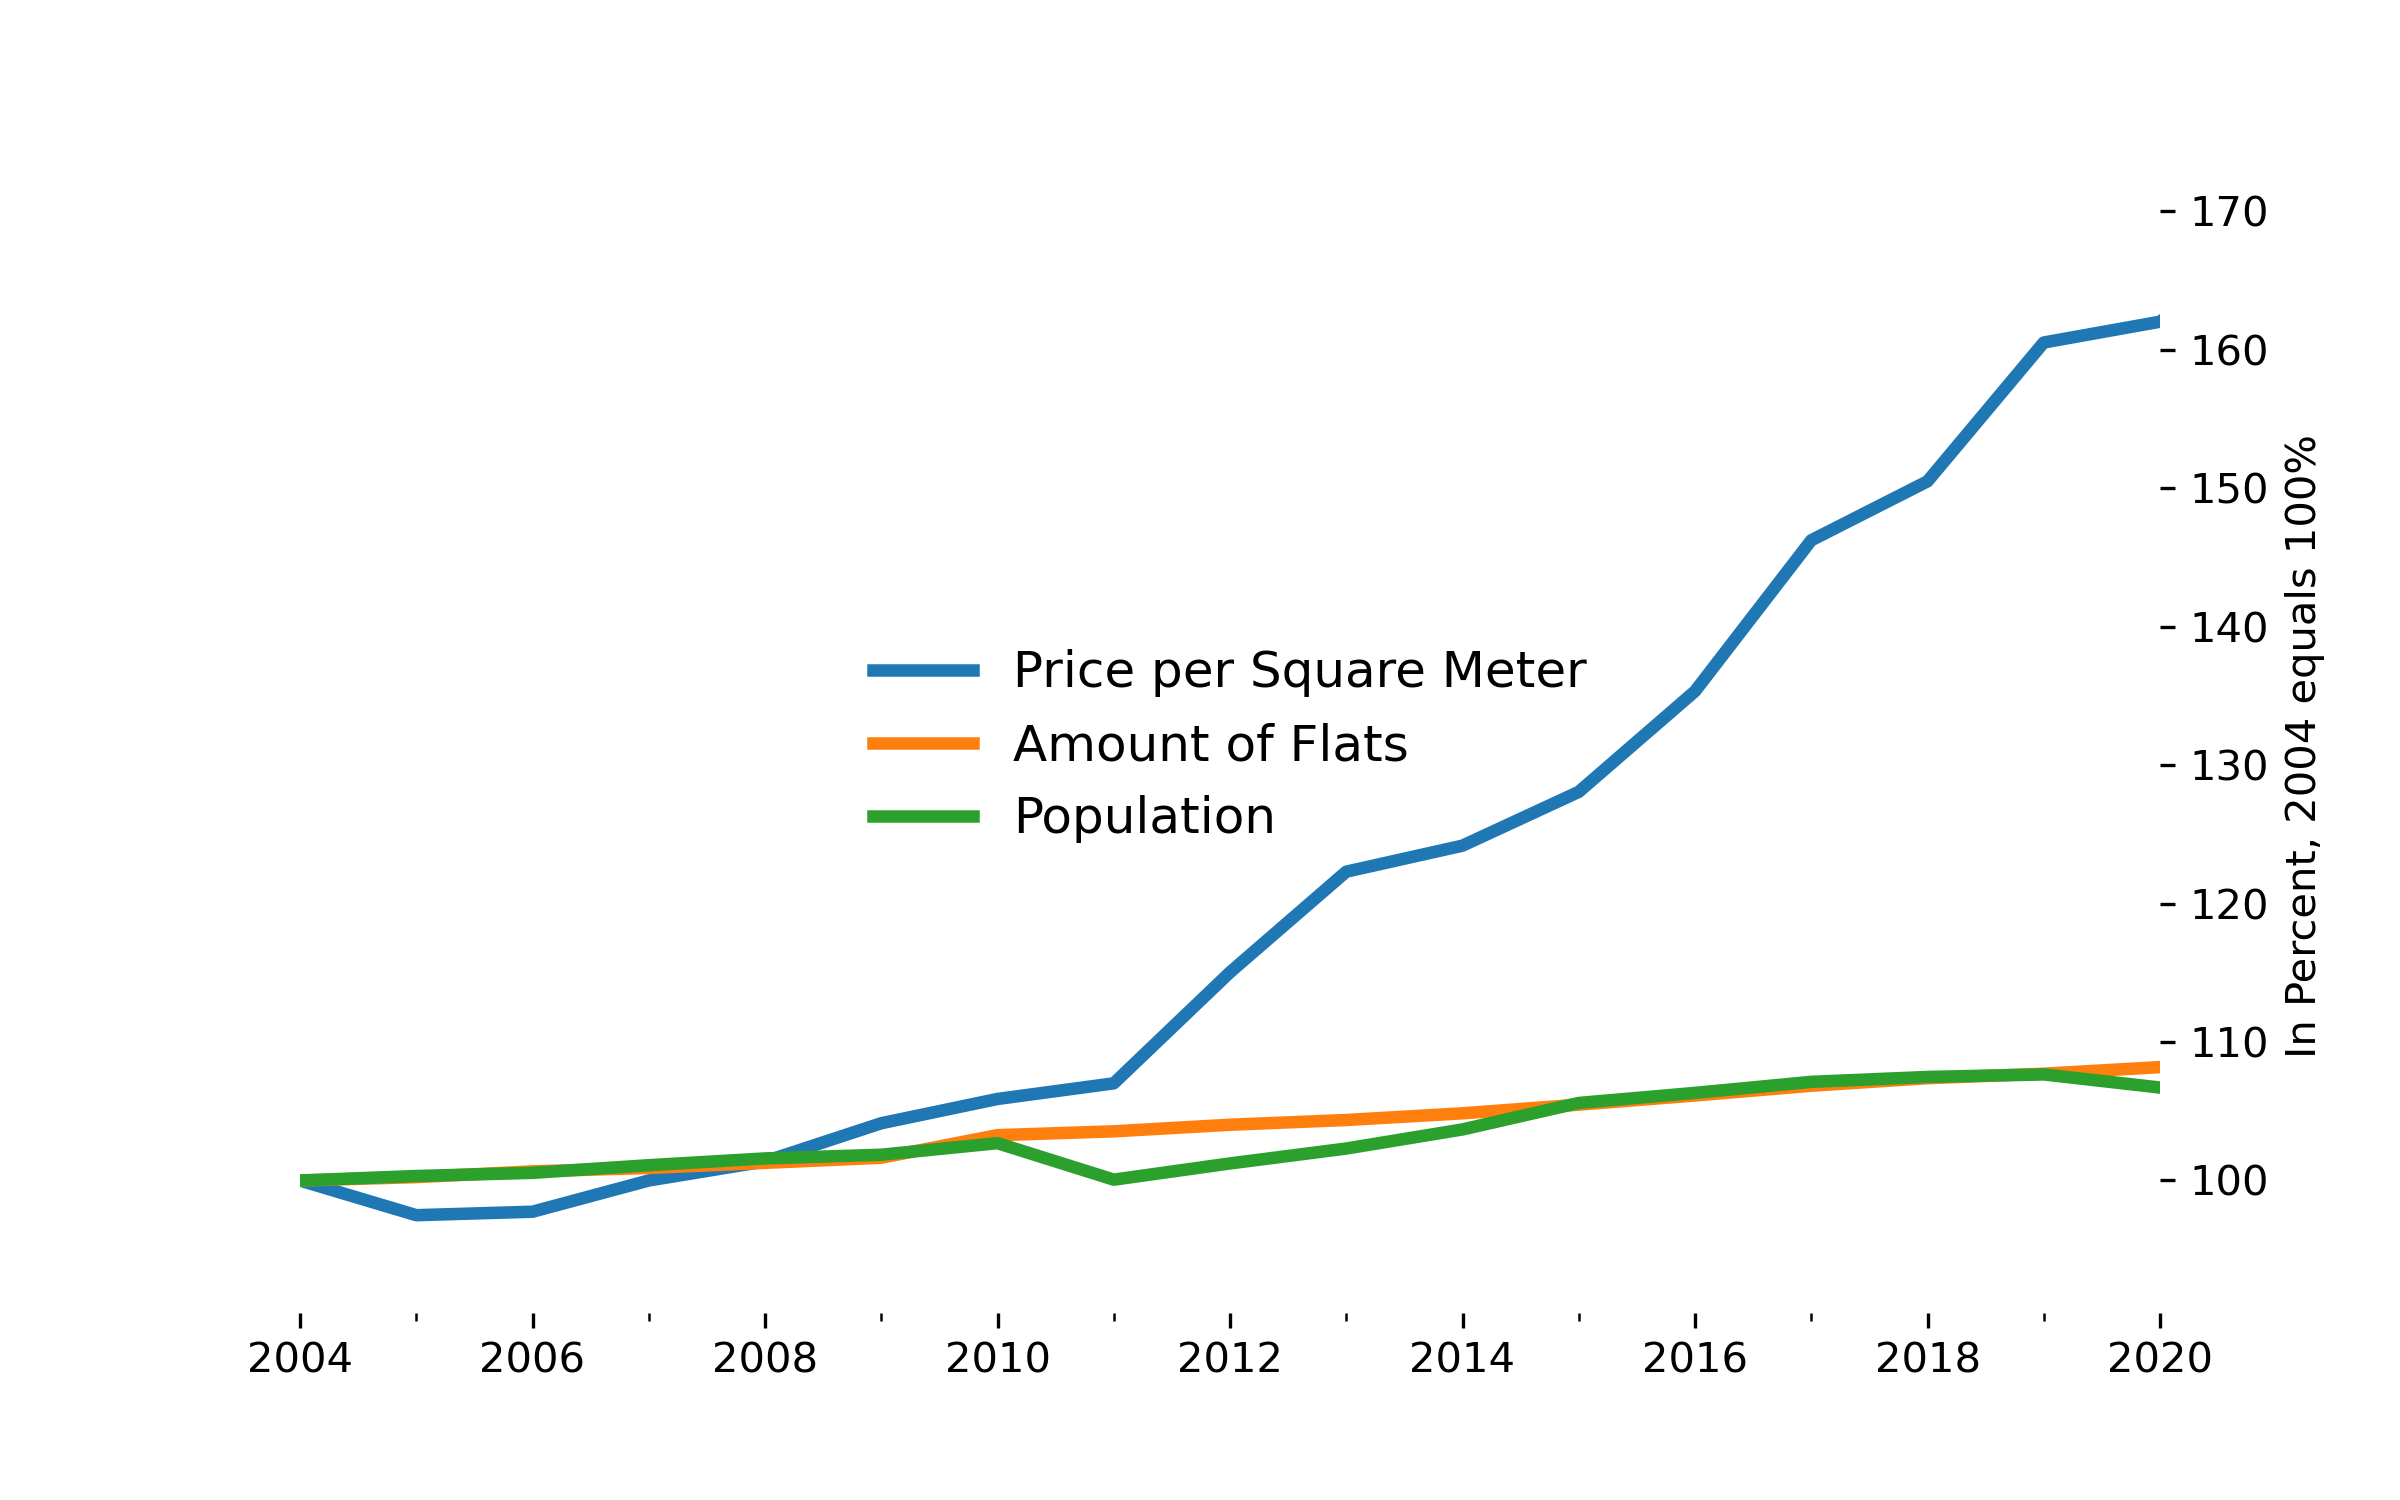
\includegraphics[width=\textwidth]{population.png}
    \caption{Population, Living Space and Square Meter Rent in Stuttgart, Germany}
    \label{thefigure}
\end{figure}


\section{Discussion}

The image in figure \ref{thefigure} shows a line graph of three different time
series over a time span from the year 2004 to 2020. The lines represent the
price per square meter (roundabout 10 square foot), the amount of flats and the
population. All time series were normed in such a way, that the year 2004
represents 100~\%. All Lines are from the City of Stuttgart.

The figure shows, that whereas the population of Stuttgart grew by roundabout
8~\% in 16 years, and the amount of flats even exceeded that growth rate
slightly with 9~\%, the prices for renting an apartment in Stuttgart have risen
by roundabout 62~\%.

Therefore this data does not support the theory, that the prices for renting an
apartment in Stuttgart have risen to to excess demand or supply shortage.

\end{document}